\documentclass[12pt,a4paper]{article}
\usepackage[english]{babel}
\usepackage[utf8]{inputenc}
\usepackage{amssymb,amsmath}
\usepackage[all]{xy}
\usepackage{url}
\usepackage{graphicx}
\usepackage{color}
\newcommand{\angstrom}{\textup{\AA}}
\color{black}
\usepackage{geometry}
\usepackage[autostyle]{csquotes}
\usepackage{tikz}
\usetikzlibrary{bayesnet}

\usepackage{dcolumn}
\usepackage{booktabs}
\usepackage{tikz}
\usetikzlibrary{positioning,shapes,arrows}
\newcolumntype{M}[1]{D{.}{.}{1.#1}}
\usepackage{upquote} % Upright quotes for verbatim code
\usepackage{fancyvrb} % verbatim replacement that allows latex
\usepackage{float}

\usepackage{amsmath}
\usepackage{algorithm}
\usepackage[noend]{algpseudocode}

\makeatletter
\def\BState{\State\hskip-\ALG@thistlm}
\makeatother

\geometry{
	a4paper,
 	left=15mm,
 	right=15mm,
 	top=10mm,
 	bottom=15mm
}

\DefineVerbatimEnvironment{Highlighting}{Verbatim}{commandchars=\\\{\}}

\newcommand{\VerbatimStringTok}[1]{\textcolor[rgb]{0.25,0.44,0.63}{{#1}}}



\begin{document}
\title{Proximal Policy Optimization Algorithm on Open-AI gym Humanoid Enviroment}
\author{Michał Ostyk-Narbutt (1854051)\\ \\ Prof. Roberto Capobianco, Artificial intelligence 2B}

\maketitle


\begin{center}

\includegraphics[width=0.5\textwidth]{img/sapienza_logo.jpg}
\end{center}
\maketitle
\tableofcontents
\clearpage
\section{Introduction}
The goal of this project was to implement the Proximal Policy Algorithm (PPO) \cite{PPO}, and train it on the OpenAI Humanoid enviroment. The Humanoid-v2 enviroment which runs on a physics engine provided by Mujoco, has 27 degrees of freedom. 

According the authors of PPO, the algorithm "perform comparably or better than state-of-the-art approaches while being much simpler to implement and tune." \cite{PPO}. Policy gradients have a convergence problem which is addressed  by the natural policy gradient (NPG) \cite{NPG}. However, NPG in practice uses a second-order derivative matrix which is hard to scale for large problems, and is computationally unfeasible. PPO on the other hand, instead of imposing a hard constraint, it  formalizes the constraint as a penalty in the "surrogate" objective function \cite{hui}. Hence, PPO may use a first-order optimizer like Gradient Descent (GD) to optimize the objective. Moreover, PPO uses multiple epochs mini-batch updates  instead of performing only one gradient update per data sample like PG methods. Another method which PPO outperforms is the Trust Region Policy Objective, which is very efficient but much more complicated and and not compatible with certain architectures.



\section{State of the Art}

\subsection{Policy gradient Methods}
The objective function or Policy loss of PG Methods is defined as: 


\begin{equation}
L^{PG}(\theta) =\hat{E_{t}} [\log \pi_{\theta} (a_t|s_t) \times \hat{{A_t}}  ] 
\end{equation}\label{eq:1}


where:
\begin{itemize}
\item  $\hat{{E_t}}$ is the expectation which indicates the empirical average over a finite batch of samples.
\item $\log \pi_{\theta} (a_t|s_t$ is the log probability of taking that action at that state 
\item $\hat{{A_t}}$ is an estimator of the advantage function, if $>0$, then this action is better than the other action possible at that state.
\end{itemize}
Through differentiating \ref{eq:1}, we obtain the policy gradient estimator which is then plugged into the Stochastic GD algorithm. Hence, pushing the agent to take actions that lead to higher rewards and avoid bad actions. However, there is a problem arising from the step size as if its too small, then the training process will be too slow. On other hand, if its too high, then there will be too much variability in the training between epochs.
Whereas PPO improves the stability of the Actor training by limiting the policy update at each training step. This is done through the Clipped Surrogate Function, which constrains the policy change in a desired range.

\subsection{Clipped Surrogate Objective}
Instead of using $\log \pi$ as in \ref{eq:1} to trace the impacts of actions, the authors introduce the following probability ratio:
\begin{equation}
r_t (\theta) =\frac{\pi_{\theta}(a_t|s_t)}{ \pi_{\theta_{old}} (a_t|s_t) }
\end{equation}
which define the the probability of action under current policy divided by the probability of the action under previous policy. Hence $r_t(\theta_{old}) = 1$.\newline
If $r_t(\theta) > 1$, then action is more probable in the current policy than the old policy. However, if $0 < r_t(\theta) < 1$, then the action is less probable for current policy than for the old one.

The resulting objective function presented in the PPO paper is:

\begin{equation}
L^{CPI}(\theta) =\hat{E_{t}} [\frac{\pi_{\theta}(a_t|s_t)}{ \pi_{\theta_{old}} (a_t|s_t) }  \hat{{A_t}}  ]  = \hat{E_{t}}[r_t (\theta)  \hat{{A_t}} ]
\end{equation}

In a situation where the action taken is much more probable in our current policy than in the old one, the lack of a constraint, leads to a large policy gradient step, and a resulting excessive policy update. Hence, there is a need to introduce a constraint which will penalize changes that lead to a ratio that will away from 1, which will ensure relatively small policy updates as the new policy can't be too different from the old one.

We could use PRO, which utilizes KL divergence constrains outside of the objective function to constraint the policy update. However, this is as previously stated in the introduction, much more complex and computationally expensive.
As a consequence, the author's of PPO introduce a clip probability ratio directly in the objective function, with its clipped surrogate objective function.
\begin{equation}
L^{CLIP}(\theta) =\hat{E_{t}} [\min(r_t (\theta) \hat{{A_t}}  , \mbox{clip}(r_t (\theta), 1 - \epsilon, 1 + \epsilon) \hat{{A_t}} ]
\end{equation}
where epsilon is a hyperparameter,and according to the paper $\epsilon = 0.2$.

Hence, we obtain two probability rations: the first being one non-clipped, and the other clipped in the $\epsilon$ ranges. Next, we take the minimum of both of these objectives, so the final objective is a lower bound of the unclipped objective. 


\begin{figure}[H]
\begin{center}
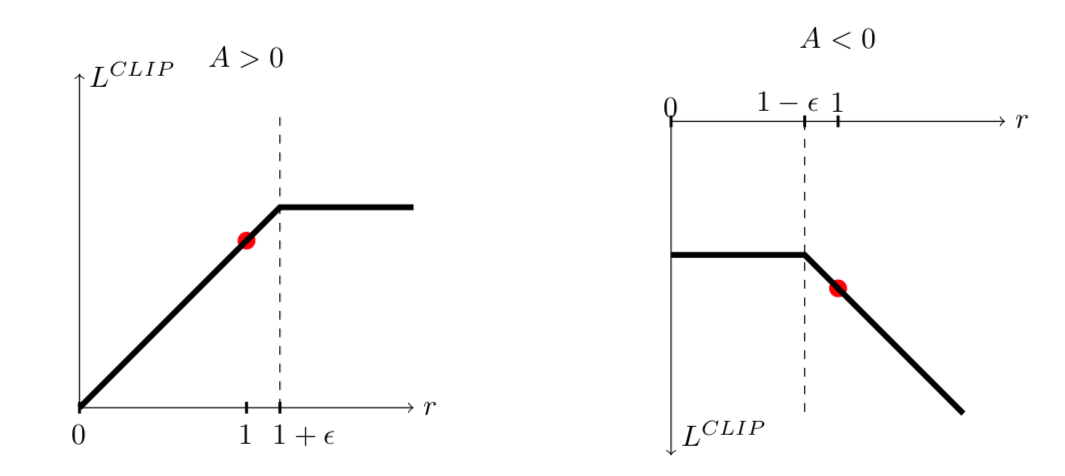
\includegraphics[width=\columnwidth, angle = 0]{img/clipped.png}
\end{center}
\caption{Plots showing one term, of the surrogate function $L^{CLIP}$ as a function of the probability ratio $r$, for positive advantages (left) and negative advantages  (right). The red circle on each plot shows the starting point for the optimization \cite{PPO}.}
\label{img:clip}
\end{figure}

Figure \ref{img:clip} presents plots of a single term in $L^{CLIP}$. \newline
\noindent In the first case when $A>0$, we want to increase the probability of taking that action at that step but not too much. However, when $A<0$, the action should be discouraged because negative effect of the outcome. Effectively, this discourages large policy change if it is outside our comfortable zone. 

When using a neural network architecture that shares parameters between the policy and value function, then there is a must to use a loss function that combines the policy surrogate and a value function error term. The addition of an entropy bonus ensures sufficient exploration.

\section{Methodology}

\subsection{Approach}
The goals of PPO can be summarised to the following:
\begin{itemize}
\item Simple and easy to implement
\item Sample efficiency
\item Minimal hyperparameter tuning
\end{itemize}

PPO includes several upgrades built on top of the Actor-Critic Algorithm. They  both seek to to maintain smooth gradient updates to get continuous improvement  and avoid unrecoverable crashes.
\begin{enumerate}
\item Generalized Advantage Estimation (GAE)$-$ a way to calculate returns which reduces variance, through  a smoothing factor $0< \lambda < 1$. The PPO paper suggests $\lambda = 0.95$.
\item Surrogate Policy loss
\item Mini-batch updates (random mini batches, and the network is gradually  updated over a fixed number of epochs)
\end{enumerate}

Algorithm \ref{euclid} depicts the overall procedure of training.
\begin{algorithm}
\caption{PPO with Clipped Objective }\label{euclid}
\begin{algorithmic}[1]
\item Collect a batch of $N$ (multiple of the mini-batch size) transitions from parallel environments \newline (state, action, log-probabilities,a reward, done-mask (0 if terminal), V(s) (value of the state for each state).
\item Calculate the returns for the batch using GAE
\item Calculate: advantage = returns - values
\item For $e$ epochs: \emph{loop}:
\begin{algorithmic}[1]
\item Sample through enough random mini-batches to cover all data.
\item Pass state into network, obtain action, value of state', entropy and new-log-probabilities.
\item Calculate the surrogate policy loss and MSE value loss.
\item Backpropagate the loss through the network using SGD.
\end{algorithmic}
\item 5. Repeat above until converged.
\end{algorithmic}
\end{algorithm}



\subsection{Implementation}

The base structure of the code, I borrowed from demo's of the  School of AI's Move37 Course \cite{code}. I made a few alterations which included the following:
\begin{itemize}
\item changed the code work with mujoco-py instead of roboschool and the humanoid-v2 enviroment
\item added several plots which will be shown in the next section containing results of the training.
\item Reimplemented the code in Tensorflow from PyTorch to gain a better understanding of the inner workings.
\end{itemize}


\section{Results}\label{results}

Since I did not have access to a dedicated GPU, I trained the model 3 times for 30 minutes, without reallly changing the hyperparameters. The results seemed constant across three runs, however, the test rewards have been increasing so I took that as a positive. The key problem with training is that the humanoid enviroment a huge observation space (376) and action space (17), resulting in slower training and more network parameters.

The results  for one of the above mentioned runs are shown in Figure \ref{img:ppo_clipped} below.

\begin{figure}[H]
\begin{center}
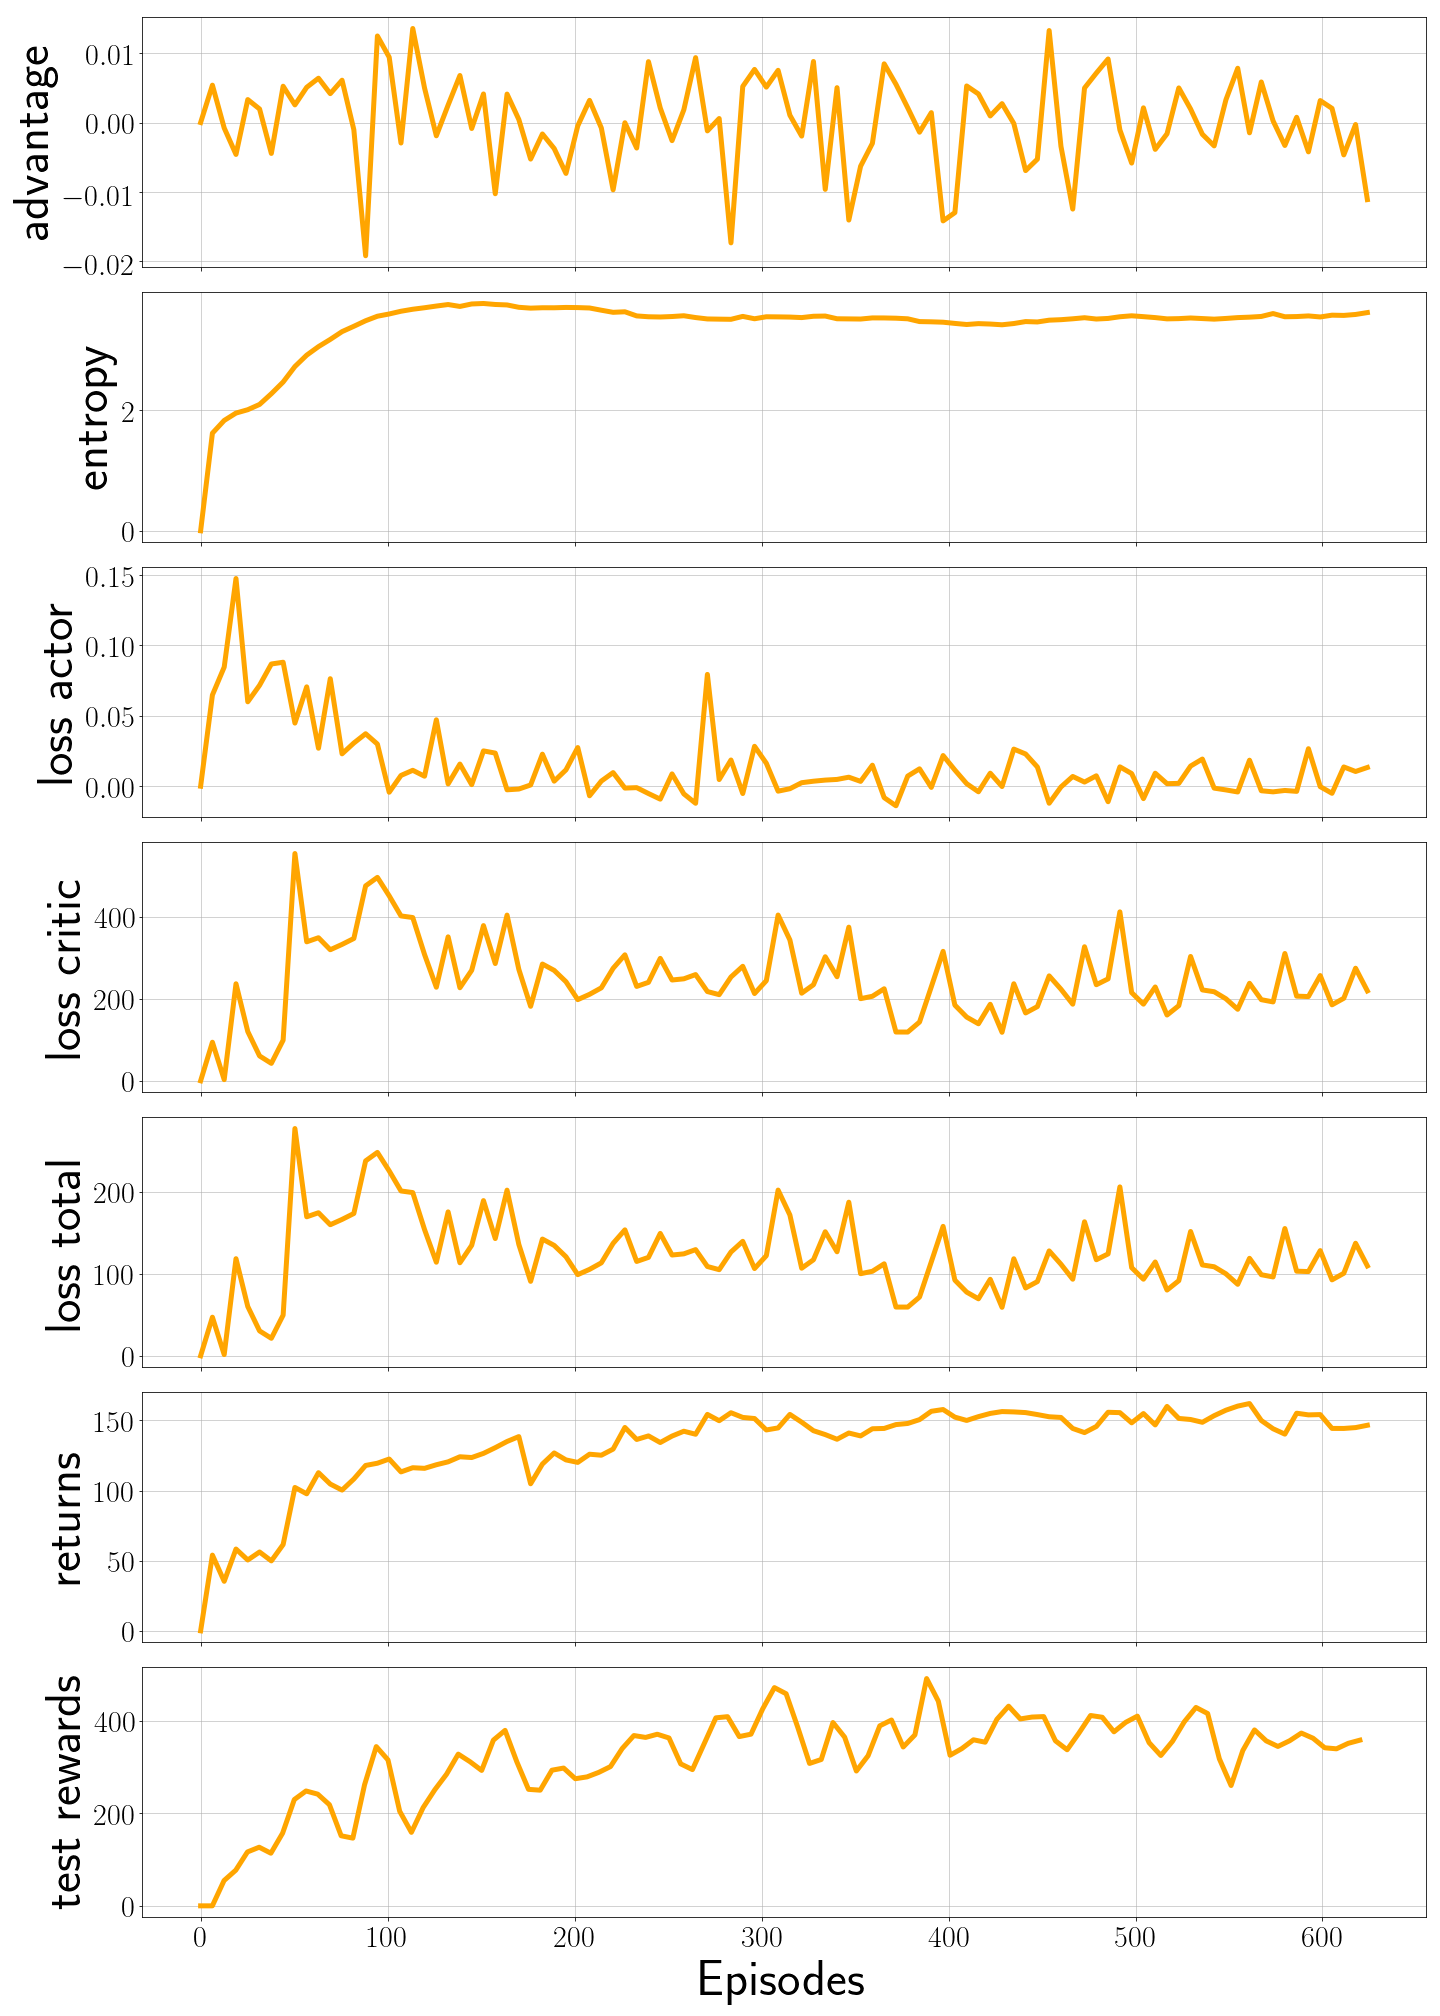
\includegraphics[width=\columnwidth, angle = 0]{img/results.png}
\end{center}
\caption{PPO with Clipped Objective  results \cite{berkley} }
\label{img:ppo_clipped}
\end{figure}

The results depict that first of all, the test rewards go gradually up and stay that way which is positive, however, then they fluctuate around the 400 score. With more training time, approximately 5-10 hours, these would probably increase more exponentially. The returns go up, and so does the entropy which would mean that the agent is making increasingly more rational decisions with each episode.  Furthermore the overall loss is decreasing as well, but stable which also results in stabilized rewards in this training run.

\section{Conclusions}

To conclude, the overall results for using the PPO algorithm with a Clipped Surrogate Objective Function, give very promising results. However, more training time, on a better workstation with a dedicated GPU is necessary to visualize proper learning and progress. The agent (humanoid) moves gradually by taking very little steps before falling over, which indicates caution and this is probably the result of the clipped range, which prohibits huge policy change. The video visualizing a couple of test runs, as well as the code, can be obtained at this Github repository \cite{code}.


\begin{thebibliography}{1}
%\bibitem{web14} Samper Zapater, J. Javier. (2014). From web 1.0 to web 4.0: the evolution of the web.

\bibitem{PPO} Schulman, John \& Wolski, Filip \& Dhariwal, Prafulla \& Radford, Alec \& Klimov, Oleg. (2017). Proximal Policy Optimization Algorithms. 
\bibitem{berkley} Joshua Achiam UC Berkeley, OpenAI \url{http://rail.eecs.berkeley.edu/deeprlcourse-fa17/f17docs/lecture_13_advanced_pg.pdf}

\bibitem{NPG} Kakade, Sham. (2001). A Natural Policy Gradient. Adv. Neural Inf. Process Syst.. 14. 1531-1538. 

\bibitem{hui} \url{https://medium.com/@jonathan_hui/rl-proximal-policy-optimization-ppo-explained-77f014ec3f12}

\bibitem{a} \url{https://towardsdatascience.com/proximal-policy-optimization-ppo-with-sonic-the-hedgehog-2-and-3-c9c21dbed5e}

\bibitem{code} \url{https://github.com/Ostyk/walk-bot}




\end{thebibliography}

\end{document}
